\documentclass[CT4S-EN-RU]{subfiles}

\begin{document}

\section{\caseENGRUS{Groups}{ / }{Группы}}\label{sec:groups}

\begin{blockENG}
Groups are monoids in which every element has an inverse. If we think of these structures in terms of how they act on sets, the difference between groups and monoids is that the action of every group element can be undone. One way of thinking about groups is in terms of symmetries. For example, the rotations and reflections of a square form a group. 
\end{blockENG}

\begin{blockRUS}
\end{blockRUS}

\begin{blockENG}
Another way to think of the difference between monoids and groups is in terms of time. Monoids are likely useful in thinking about diffusion, in which time plays a role and things cannot be undone. Groups are more likely useful in thinking about mechanics, where actions are time-reversible. 
\end{blockENG}

\begin{blockRUS}
\end{blockRUS}

%%%% Subsection %%%%

\subsection{\caseENGRUS{Definition and examples}{ / }{Определение и примеры}}

\begin{definitionENG}\label{def:group}\index{group}\index{monoid!inverse of an element in}
Let $(M,e,\star)$ be a monoid. An element $m\in M$ is said to {\em have an inverse} if there exists an $m'\in M$ such that $mm'=e$ and $m'm=e$. A {\em group} is a monoid $(M,e,\star)$ in which every element $m\in M$ has an inverse.
\end{definitionENG}

\begin{definitionRUS}\label{def:group}\index{group}\index{monoid!inverse of an element in}
\end{definitionRUS}

\begin{propositionENG}
Suppose that $\mcM:=(M,e,\star)$ is a monoid and let $m\in M$ be an element. Then $m$ has at most one inverse.
\footnote{If $\mcM$ is a group then every element $m$ has exactly one inverse.}
\end{propositionENG}

\begin{propositionRUS}
\end{propositionRUS}

\begin{proofENG}
Suppose that both $m'$ and $m''$ are inverses of $m$; we want to show that $m'=m''$. This follows by the associative law for monoids:
$$m'=m'(mm'')=(m'm)m''=m''.$$
\end{proofENG}

\begin{proofRUS}
\end{proofRUS}

\begin{exampleENG}
The additive monoid $(\NN,0,+)$ is not a group because none of its elements are invertible, except for $0$. However, the monoid of integers $(\ZZ,0,+)$ is a group. The monoid of clock positions from Example \ref{ex:cyclic} is also a group. For example the inverse of $Q^5$ is $Q^7$ because $Q^5\star Q^7=e=Q^7\star Q^5$.
\end{exampleENG}

\begin{exampleRUS}
\end{exampleRUS}

\begin{exampleENG}
Consider a square centered at the origin in $\RR^2$. It has rotational and mirror symmetries. There are eight of these, which we denote $$\{e,\rho,\rho^2,\rho^3,\phi,\phi\rho,\phi\rho^2,\phi\rho^3\},$$ where $\rho$ stands for $90^\circ$ counterclockwise rotation and $\phi$ stands for horizontal-flip (across the vertical axis). So relations include $\rho^4=e$, $\phi^2=e$, and $\rho^3\phi=\phi\rho$.
\end{exampleENG}

\begin{exampleRUS}
\end{exampleRUS}

\begin{exampleENG}\label{ex:important groups}
The set of $3\times 3$ matrices can be given the structure of a monoid, where the identity element is the $3\times 3$ identity matrix, the multiplication is matrix multiplication. The subset of invertible matrices forms a group, called {\em the general linear group of dimension 3}\index{a group!$GL_3$} and denoted $GL_3$. Inside of $GL_3$ is the so-called {\em orthogonal group}, denoted $O_3$, of matrices $M$ such that $M^\m1=M^\top$. These matrices correspond to symmetries of the sphere centered at the origin.

Another interesting group is the Euclidean group\index{a group!$E_3$} $E(3)$ which consists of all {\em isometries} of $\RR^3$, i.e. all functions $\RR^3\to\RR^3$ that preserve distances.  
\end{exampleENG}

\begin{exampleRUS}\label{ex:important groups}
\end{exampleRUS}

\begin{applicationENG}\label{app:groups for symmetry}\index{symmetry}
In \href{http://en.wikipedia.org/wiki/Crystallography}{\text crystallography} one is often concerned with the symmetries that arise in the arrangement $A$ of atoms in a molecule. To think about symmetries in terms of groups, we first define an {\em atom-arrangement} to be a finite subset $i\taking A\ss\RR^3$. A symmetry in this case is an isometry of $\RR^3$ (see Example \ref{ex:important groups}), say $f\taking\RR^3\to\RR^3$ such that there exists a dotted arrow making the diagram below commute:
$$
\xymatrix{A\ar@{-->}[r]\ar[d]_i&A\ar[d]^i\\\RR^3\ar[r]_f&\RR^3}
$$
That is, it's an isometry of $\RR^3$ such that each atom of $A$ is sent to a position currently occupied by an atom of $A$. It is not hard to show that the set of such isometries forms a group, called the \href{http://en.wikipedia.org/wiki/Space_group}{\em space group}\index{space group} of the crystal.
\end{applicationENG}

\begin{applicationRUS}\label{app:groups for symmetry}\index{symmetry}
\end{applicationRUS}

\begin{exerciseENG}\label{exc:permutation}\index{set!permutation of}
Let $S$ be a finite set. A {\em permutation of $S$}\index{permutation} is an isomorphism $f\taking S\To{\iso}S$. 
\begin{center}
\parbox{2.3in}{
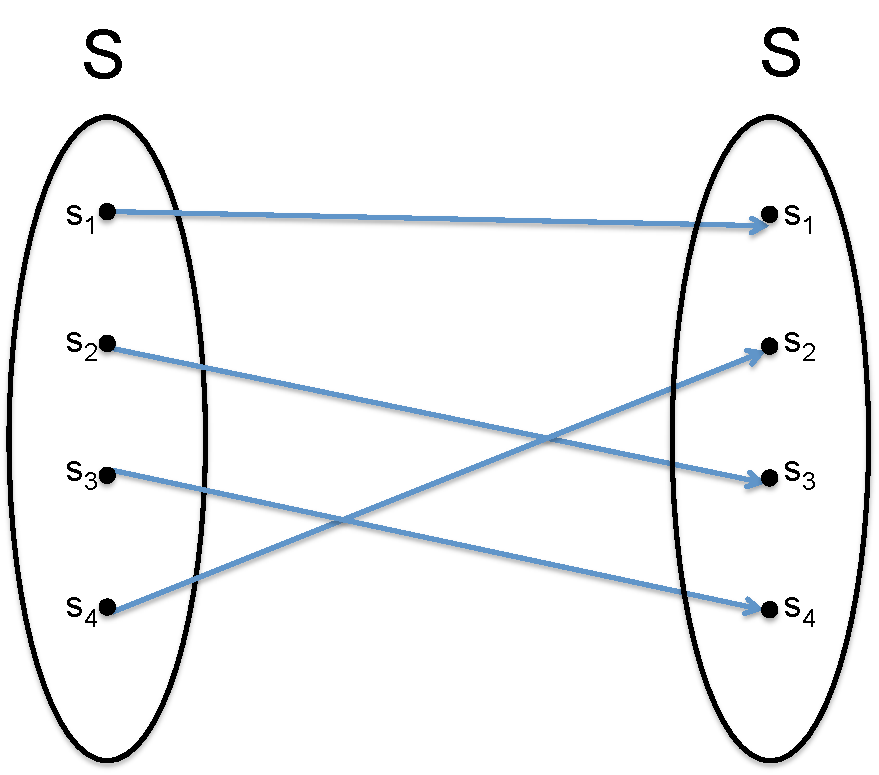
\includegraphics[height=2in]{SetPermutation}}
\end{center}
\sexc Come up with an identity, and a  multiplication formula, such that the set of permutations of $S$ forms a monoid. 
\item Is it a group?
\endsexc
\end{exerciseENG}

\begin{exerciseRUS}\label{exc:permutation}\index{set!permutation of}
\end{exerciseRUS}

\begin{exerciseENG}
In Exercise \ref{exc:classify cyclic} you classified the cyclic monoids. Which of them are groups? 
\end{exerciseENG}

\begin{exerciseRUS}
\end{exerciseRUS}

\begin{definitionENG}[Group action]\label{def:group action}\index{group!action}\index{action!of a group}
Let $(G,e,\star)$ be a group and $S$ a set. An {\em action} of $G$ on $S$ is a function $\acts\taking G\times S\to S$ such that for all $s\in S$ and $g,g'\in G$, we have
\begin{itemize}
\item $e\acts s=s$ and
\item $g\acts(g'\acts s)=(g\star g')\acts s.$
\end{itemize}
In other words, considering $G$ as a monoid, it is an action in the sense of Definition \ref{def:monoid action}.
\end{definitionENG}

\begin{definitionRUS}[Group action]\label{def:group action}\index{group!action}\index{action!of a group}
\end{definitionRUS}

\begin{exampleENG}\label{ex:U(1)}\index{a group!$U(1)$}
When a group acts on a set, it has the character of \href{http://en.wikipedia.org/wiki/Symmetry}{\text symmetry}. For example, consider the group whose elements are angles $\theta$. This group may be denoted $U(1)$ and is often formalized as the unit circle in $\CC$ of complex numbers $z=a+bi$ such that $|z|=a^2+b^2=1$. The set of such points is given the structure of a group $(U(1),e,\star)$ by defining the identity element to be $e:=1+0i$ and the group law to be complex multiplication. But for those unfamiliar with complex numbers, this is simply angle addition where we understand that $360^\circ=0^\circ$. If $\theta_1=190^\circ$ and $\theta_2=278^\circ$, then $\theta_1\star\theta_2=468^\circ=108^\circ.$ In the language of complex numbers, $z=e^{i\theta}$.

The group $U(1)$ acts on any set that we can picture as having rotational symmetry about a fixed axis, such as the earth around the north-south axis. We will define $S=\{(x,y,z)\in\RR^3\|x^2+y^2+z^2=1\}$, the unit sphere, and understand the rotational action of $U(1)$ on $S$.\index{orbit!rotating earth}

We first show that $U(1)$ acts on $\RR^3$ by $\theta\acts(x,y,z)=(x\cos\theta+y\sin\theta, -x\sin\theta+y\cos\theta,z)$, or with matrix notation as 
$$\theta\acts(x,y,z)
:=(x,y,z)\left(\begin{array}{ccc}
\cos(\theta)&-\sin(\theta)&0\\
\sin(\theta)&\cos(\theta)&0\\
0&0&1\end{array}\right)
$$
\href{http://en.wikipedia.org/wiki/List_of_trigonometric_identities#Matrix_form}{\text Trigonometric identities} ensure that this is indeed an action.

In terms of action tables, we would need infinitely many columns to express this action. Here is a sample
$$
\begin{tabular}{| l || l | l | l |}
\bhline
\multicolumn{4}{|c|}{Action of $U(1)$ on $\RR^3$}\\\bhline
{$\RR^3$}&{$\theta=45^\circ$}&{$\theta=90^\circ$}&{$\theta=100^\circ$}\\\bbhline
(0,0,0)&(0,0,0)&(0,0,0)&(0,0,0)\\\hline
(1,0,0)&(.71,.71,0)&(0,1,0)&(-.17,.98,0)\\\hline
(0,1,-4.2)&(-.71,.71,-4.2)&(-1,0,-4.2)&(-.98,-.17,-4.2)\\\hline
(3,4,2)&(4.95,.71,2)&(-4,3,2)&(3.42,-3.65,2)\\\hline
$\vdots$&$\vdots$&$\vdots$&$\vdots$\\\bhline
\end{tabular}
$$

Finally, we are looking to see that the action preserves length so that if $(x,y,z)\in S$ then $\theta\acts(x,y,z)\in S$; this way we will have confirmed that $U(1)$ indeed acts on $S$. The calculation begins by assuming $x^2+y^2+z^2=1$ and checks 
$$
(x\cos\theta+y\sin\theta)^2+(-x\sin\theta+y\cos\theta)^2+z^2=x^2+y^2+z^2=1.
$$
\end{exampleENG}

\begin{exampleRUS}\label{ex:U(1)}\index{a group!$U(1)$}
\end{exampleRUS}

\begin{exerciseENG}\label{exc:permutation group}
Let $X$ be a set and consider the group of permutations of $X$ (see Exercise \ref{exc:permutation}), which we will denote $\Sigma_X$\index{a group!$\Sigma_X$}. Find a canonical action of $\Sigma_X$ on $X$.
\end{exerciseENG}

\begin{exerciseRUS}\label{exc:permutation group}
\end{exerciseRUS}

\begin{definitionENG}
Let $G$ be a group acting on a set $X$. For any point $x\in X$, the {\em orbit of $x$},\index{orbit}\index{action!orbit of} denoted $Gx$, is the set 
$$Gx:=\{x'\in X\|\exists g\in G \tn{ such that }gx=x'\}.$$
\end{definitionENG}

\begin{definitionRUS}
\end{definitionRUS}

\begin{applicationENG}
Let $S$ be the surface of the earth, understood as a sphere, and let $G=U(1)$ be the group of angles acting on $S$ as in Example \ref{ex:U(1)}. The orbit of any point $p=(x,y,z)\in S$ is the set of points on the same latitude line as $p$.

One may also consider a small band around the earth, i.e. the set $A=\{(x,y,z)\|1.0\leq x^2+y^2+z^2\leq 1.05\}$. The action of $U(1)\acts S$ extends to an action $U(1)\acts A$. The orbits are latitude-lines-at-altitude. A simplifying assumption in \href{http://en.wikipedia.org/wiki/Climatology}{\text climatology} may be given by assuming that $U(1)$ acts on all currents in the atmosphere in an appropriate sense. That way, instead of considering movement within the whole space $A$, we only allow movement that behaves the same way throughout each orbit of the group action.
\end{applicationENG}

\begin{applicationRUS}
\end{applicationRUS}

\begin{exerciseENG}~
\sexc Consider the $U(1)$ action on $\RR^3$ given in Example \ref{ex:U(1)}. Describe the set of orbits of this action.
\item What are the orbits of the action of the permutation group $\Sigma_{\{1,2,3\}}$ on the set $\{1,2,3\}$? (See Exercise \ref{exc:permutation group}.)
\endsexc
\end{exerciseENG}

\begin{exerciseRUS}~
\end{exerciseRUS}

\begin{exerciseENG}
Let $G$ be a group and $X$ a set on which $G$ acts by $\acts\taking G\times X\to X$. Is “being in the same orbit” an equivalence relation on $X$? 
\end{exerciseENG}

\begin{exerciseRUS}
\end{exerciseRUS}

\begin{definitionENG}\label{def:group homomorphism}\index{group!homomorphism of}
Let $G$ and $G'$ be groups. A {\em group homomorphism} $f\taking G\to G'$ is defined to be a monoid homomorphism $G\to G'$, where $G$ and $G'$ are being regarded as monoids in accordance with Definition \ref{def:group}.
\end{definitionENG}

\begin{definitionRUS}\label{def:group homomorphism}\index{group!homomorphism of}
\end{definitionRUS}

\end{document}
